\documentclass[lettersize,journal]{IEEEtran}
\usepackage{amsmath,amsfonts}
\usepackage{algorithmic}
\usepackage{algorithm}
\usepackage{array}
\usepackage[caption=false,font=normalsize,labelfont=sf,textfont=sf]{subfig}
\usepackage{subcaption}
\usepackage{textcomp}
\usepackage{stfloats}
\usepackage{url}
\usepackage{verbatim}
\usepackage{graphicx}
\usepackage{tikz}
\usetikzlibrary{automata, positioning}
\usepackage{cite}
\hyphenation{op-tical net-works semi-conduc-tor IEEE-Xplore}
% updated with editorial comments 12/2/2022

\begin{document}

\title{Journal DAO: \\ User-Incentivized Autonomous Decentralized Scientific Publishing in Web3}

\author{Tai Jiang, Rui Qin,~\IEEEmembership{Member, IEEE}, Yuhang Liu, \\
 Fei-YueWang,~\IEEEmembership{Fellow,~IEEE}.
        % <-this % stops a space
\thanks{This work was supported by the Science and Technology Development Fund of Macau SAR under Grant 0093/2023/RIA2 and  Grant 0050/2020/A1.}% <-this % stops a space
\thanks{Manuscript received February 15, 2023; revised February 15, 2023.}
\thanks{Tai Jiang is with the Department of Engineering Science, Faculty of Innovation Engineering, Macau University of Science and Technology, Macao, 999078, China (e-mail: jiangtai20@mails.ucas.ac.cn).}
\thanks{Rui Qin is with the State Key Laboratory for Management and Control of Complex Systems and the State Key Laboratory of Multimodal Artificial Intelligence Systems, Institute of Automation, Chinese Academy of Sciences, Beijing 100190, China (e-mail: rui.qin@ia.ac.cn).}
\thanks{Yuhang Liu is with the State Key Laboratory for Management and Control of Complex Systems, Institute of Automation, Chinese Academy of Sciences, Beijing 100190, China, and also with the School of Artificial Intelligence, University of Chinese Academy of Sciences, Beijing 100049, China (e-mail: liuyuhang21@mails.ucas.ac.cn).}
\thanks{Fei-Yue Wang is with the State Key Laboratory for Management and Control of Complex Systems, Chinese Academy of Sciences, Beijing 100190, China, and also with the Macao Institute of Systems Engineering, Macau University of Science and Technology, Macao 999078, China (e-mail: feiyue.wang@ia.ac.cn).}

}

% The paper headers
\markboth{Journal of \LaTeX\ Class Files,~Vol.~14, No.~8, February~2023}%
{Shell \MakeLowercase{\textit{et al.}}: A Sample Article Using IEEEtran.cls for IEEE Journals}

% \IEEEpubid{0000--0000/00\$00.00~\copyright~2021 IEEE}
% Remember, if you use this you must call \IEEEpubidadjcol in the second
% column for its text to clear the IEEEpubid mark.

\maketitle

\begin{abstract}

The academic publishing industry is currently undergoing significant growth but also faces several challenges, mainly including the lack of transparency in the peer review process and the limited rights of authors. The rise of Web3, emphasizing decentralization, openness, and user control over data, opens up new perspectives for academic publishing. This article introduces an innovative academic publishing model, named Journal DAO, leveraging emerging Web3 technologies such as blockchain and decentralized autonomous organization (DAO). First, by recording articles on the blockchain rather than a specific database, Journal DAO can ensure data security and traceability of the articles. Second, through the governance framework of DAO, tokens are distributed among all the participants of Journal DAO based on the their contributions, safeguarding the rights of each role in the publishing process. Third, effective incentive mechanisms are proposed to reward all participants, ensuring the sustainability of the framework and its autonomous functionality. This work proposes a prospective academic publishing model that aims to reshape the industry through the application of blockchain and DAO in Web3, making a significant contribution to future academic publishing.


\end{abstract}


\begin{IEEEkeywords}
decentralized autonomous organizations, blockchain, Web3, decentralized funding, decentralized science
\end{IEEEkeywords}

\section{Introduction \label{sec:introduction}}


\IEEEPARstart{T}{he} academic publishing industry is currently facing several pressing challenges. First, the traditional system, often conducted anonymously, fails to ensure fairness and impartiality, leading to a compromised review process that undermines both credibility and integrity. This lack of transparency can undermine the credibility and integrity of the review process. Second,
the authors often lack control over associated data of their articles, since the ownership often rests with publishers or electronic databases. This challenges authors in retaining rights, deciding on data use, and hampers their ability to fully leverage research, limiting collaborative opportunities and further advancements in their field. Third, the restrictions on data sharing hinder the free flow of knowledge and inhibit potential collaborations, which limits authors from fully benefiting and making discoveries that could contribute to the scientific community.

The emergence of technologies such as Decentralized Autonomous Organizations (DAOs) \cite{buterin2014next} and blockchain \cite{swan2015blockchain,9093840} presents significant opportunities for the advancement of the academic publishing industry. DAOs offer a groundbreaking approach to organizational governance, decision-making, and fund management for academic publishing \cite{wang2019decentralized}. Unlike traditional hierarchical structures, DAOs operate without central authorities, relying on transparent and automated processes governed by smart contracts and consensus protocols \cite{kaal2021decentralized}. This decentralization can provide a transparent and auditable decision-making process, enhance accountability, and facilitate efficient funds distribution for the current academic publishing system. The decentralized and tamper-resistant nature of blockchain can provide a secure and transparent environment for intelligent journals. By integrating blockchain technology into intelligent journals, the data transparency and authenticity can be realized. Through blockchain-based smart contracts, the reliability of data can be steadfastly guaranteed, thereby eliminating the necessity for third-party oversight \cite{mougayar2016business}. This innovative approach not only enhances the credibility of information but also streamlines the process, fostering trust and efficiency within the realm of intelligent journals.

In the literature, the applications of blockchain-based decentralized technologies in academic publishing have received researchers' great attention \cite{8756390}. Blockchain technology was used to solve the security and efficiency concerns in the distribution and management of open journal systems, ensuring precise distribution, enhancing reputation and trust, and safeguarding paper management against potential hacker threats \cite{agustin2020blockchain}. Through decentralized InterPlanetary File System (IPFS) and blockchain technologies, the authenticity, trust and reliability of online publications can be ensured, which can effectively address the challenges related to security and privacy in online publications \cite{nizamuddin2018ipfs}. By leveraging blockchain-based decentralized technologies, a decentralized scientific publishing platform is established, which utilizes Ethereum smart contracts to expedite the publication process, reduce biases in peer review, and lower publication costs \cite{becstacs2023novel}. The platform can ensure complete traceability throughout the publication processes, and all the participants including the editors, reviewers, and authors will receive system tokens as rewards for their contributions.

However, these existing studies primarily concentrate on specific aspects, such as the use of blockchain to address security and efficiency concerns or enhance transparency in the academic publishing process. They do not comprehensively address the multifaceted challenges prevalent in the current academic publishing landscape. This article proposes an innovative academic publishing model called Journal DAO, which applies emerging Web3 technologies, such as blockchain and DAO, to address these challenges. First, by recording articles on the blockchain, all operations are conducted on the chain rather than belonging to a specific database, ensuring data security and traceability. Second, through the DAO framework, tokens are distributed based on role contributions, protecting the rights of researchers. Third, by designing effective incentive mechanisms, with the consideration of rewarding each participant according to their contributions to the article, which can realize a fully autonomous and economically sustainable Journal DAO ecosystem \cite{ding2022desci}.

The rest of this paper is arranged as follows. Section \ref{sec:framework} introduces the framework of Journal DAO framework. Section \ref{sec:mechanism} discusses the design and implementation of the incentive mechanism in Journal DAO. Section \ref{sec:performance} presents experimental results validating the effectiveness of the implemented incentive mechanism.
Section \ref{sec:conclusion} concludes the paper.

% 第2节之前的内容共1.25页

\section{Framework of Journal DAO \label{sec:framework}}

% 第2节共2.25页
% 开头写一段话,介绍本节主要做什么,2-3行即可。




% \subsection{The Framework}1页

% 本小节给出Journal DAO的framework,建议画一张框架图,图中要包含所有参与者,还要包含完整的运行流程,以及token和finance的流转。

% 在框架图的基础上,简要介绍框架图,并说明区块链和DAO在其中如何发挥作用。

% \subsection{The Operation Process}1页

% 介绍Journal DAO框架中参与者的各类角色,Journal DAO运行流程和实现的功能,以及token和finance如何流转。

% \subsection{The Advantages}0.25页

% 介绍与传统期刊相比,Journal DAO有哪些优势.

% \section{Mechanism Design of Journal DAO \label{sec:mechanism}}本节共2页
% 简要写一下本节的思路,3-5行即可。

% \subsection{Decentralized Governance}

% \subsection{Initial Token Distributions}

% \subsection{Token Distributions upon Article Download or Citation}

% \subsection{Finance Distributions}

% \section{A Case Study} \label{sec:performance}本节共2页

% \section{Conclusions and Future Work\label{sec:conclusion}}共0.25页

% 第一段,对本文的工作进行总结。

% 第二段,对下一步的工作进行展望。

% \bibliography{refs}1页
% \bibliographystyle{IEEEtran}

% 作者简介:0.75页





\begin{figure}[h!]
  \centering
  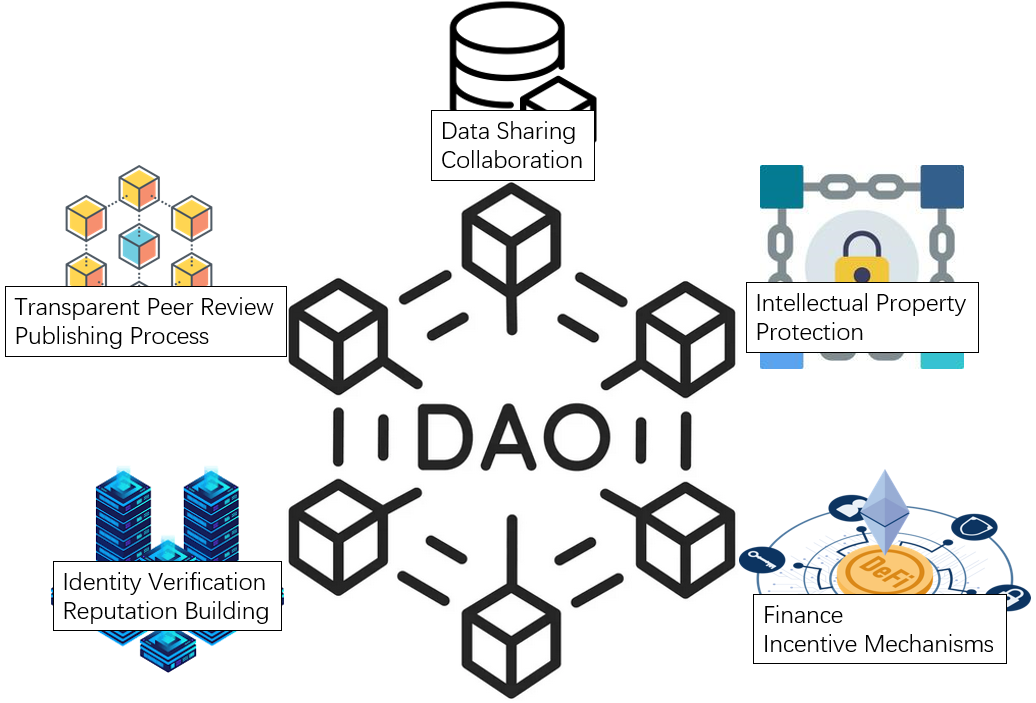
\includegraphics[width=\linewidth]{assets/dao.png}
  \caption{Application of DAO in Article and Journal}
  \label{fig:applicationofdao}
\end{figure}


According to the development of district DAO, related blockchain technology, the following DAO to Decentralized Scientific (DeSci) framework can be summarized as shown in the figure \ref{fig:applicationofdao}.It aims to establish a decentralized scientific publishing platform using blockchain and smart contract technology \cite{szabo1996smart}, enabling fair, transparent, and efficient scientific research dissemination \cite{wang2022dao}\cite{10394624}\cite{shilina2023decentralized}.
%按照区DAO,以及相关区块链技术的发展,可以如图总结出以下的DAO框架。它旨在通过区块链和智能合约技术,建立一个去中心化的科学出版平台,实现科学研究的公平、透明和高效。

\begin{itemize}
  \item \textbf{Transparent Peer Review and Publishing Process:} 
  
  Blockchain can be used to create a transparent academic publishing platform, ensuring transparency throughout the peer-review and publishing processes.\cite{nakamoto2008bitcoin} Smart contracts can manage review, publication, and payment procedures, ensuring traceability and fairness.
  %透明的学术出版: 区块链可以用于创建透明的学术出版平台,确保审稿和出版过程的透明性。智能合约可以管理审稿、出版和付款流程,确保可追溯和公平。

  \item \textbf{Protection of Intellectual Property:}
  
  Blockchain and smart contracts can safeguard authors' intellectual property, ensuring their works are not copied or distributed without permission \cite{gurkaynak2018intellectual}.
  %知识产权保护: 区块链和智能合约可用于保护作者的知识产权,确保其作品不会未经许可就被复制或传播。
  
  \item \textbf{Identity Verification and Reputation Building:} 
  
  Blockchain can be employed to establish scholars' identities and reputations \cite{radziwill2018blockchain}. Smart contracts can automate the validation of scholars' achievements, storing them on the blockchain.
  %身份验证和声誉建立: 区块链可用于建立学者的身份和声誉。智能合约可以自动化验证学者的成就,并将其存储在区块链上。
  
  \item \textbf{Data Sharing and Collaboration:} 
  
  Blockchain and smart contracts can facilitate data sharing and collaboration among scholars, ensuring data integrity and traceability \cite{praitheeshan2019security}.
  %数据共享和合作: 区块链和智能合约可用于促进学者之间的数据共享和合作,确保数据的完整性和来源可追溯。
  
  \item \textbf{Finance and Incentive Mechanisms:} 
  
  DAO and cryptocurrencies can be used to support research finance and incentive mechanisms.Funds can be allocated according to token weights \cite{schar2021decentralized}.
  %金融和激励机制: 区块链和加密货币可以用于支持学术研究的融资和激励机制。资金可以按照token为权重分配。
\end{itemize}

These application examples highlight the potential value of blockchain, smart contracts, and DAO technology in academic publishing and journal management. They enhance transparency, protect intellectual property, verify identity, automate processes, and encourage collaboration. As these technologies continue to evolve, they hold promise for further innovation and efficiency in academia \cite{vacca2021systematic}.
%这些应用示例突显了区块链、智能合约和DAO技术在学术出版和杂志管理方面的潜在应用,提高了透明度、知识产权保护、身份验证和自动化审稿流程。随着这些技术的不断发展,它们将有望为学术界提供更多的创新和效率。


\subsection{The Framework with Blockchain and DAO}
% \subsection{The Framework}1页
% 本小节给出Journal DAO的framework,建议画一张框架图,图中要包含所有参与者,还要包含完整的运行流程,以及token和finance的流转。
% 在框架图的基础上,简要介绍框架图,并说明区块链和DAO在其中如何发挥作用。

Based on the depicted framework in Figure \ref{fig:frameworkofblockchain}, it is evident that the operational flow of the blockchain and DAO framework, along with the roles of various participants \cite{10459713}, can be succinctly understood. 

\begin{figure}[h!]
  \centering
  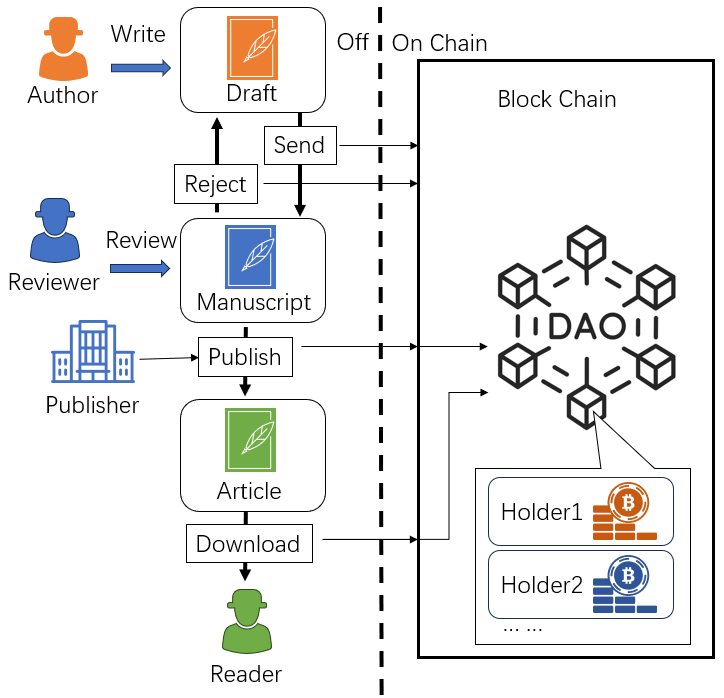
\includegraphics[width=\linewidth]{assets/workflow.png}
  \caption{Framework of Blockchain.}
  \label{fig:frameworkofblockchain}
\end{figure}


Initially, authors generate manuscripts that can be submitted for publication. However, unlike conventional websites where manuscripts reside solely on publishing servers, this framework ensures their credibility by immutably recording the publication process on the blockchain. 

Subsequently, manuscripts undergo a rigorous peer review process, involving multiple reviewers who diligently evaluate them. Only manuscripts that successfully pass the review are considered for publication. In cases where revisions are necessary, manuscripts are returned to the authors accompanied by specific feedback. Importantly, this entire review process is transparently recorded on the blockchain, thereby ensuring objectivity and effectiveness in the evaluation. 
In the event of manuscript rejection, authors have the opportunity to resubmit their work for publication, with this resubmission process meticulously documented on the blockchain. This traceability feature guarantees complete transparency throughout the submission process. 

Upon successful completion of the review process, approved manuscripts are published. This publication is also recorded on the blockchain and subsequently integrated into the DAO framework, where contribution allocation occurs in accordance with established procedures \cite{hsieh2018bitcoin}. 
Readers can access and download published articles, with this downloading process also being recorded on the blockchain. Such a record ensures an accurate reflection of article downloads and citations. Furthermore, downloads and citations are incorporated into the DAO framework, facilitating the equitable allocation of contributions. Readers, being pivotal in determining the value of articles, receive corresponding contributions within the framework.
% 根据图1中的框架,可以简单的看出区块链和DAO的框架的运行流程,以及各个参与者的角色在框架中的作用。首先,作者撰写了文章,可以发布手稿。发布之后,不是跟传统网站一样,只存在了出版上的服务器中,这个过程会上链,保证了文章的可信性。然后,手稿进入了审稿流程,多个审稿人对文章进行了审查,通过了审查,才能发布出版。如果需要修改,会退还给作者,并且附上修改意见,这个过程也会上链,保证了评审的客观有效。被退回的文章会被重新发布,这个过程依然上链,整个申购流程完全透明可回溯。最后,文章被通过了审查,会被发表出版,这个过程也会上链,并且上链之后,进入了DAO框架,按照流程进行贡献分配。读者可以下载发布后的文章,这个过程也会上链,能真实反映文章的下载以及引用。并且下载以及引用之后,也会进入DAO框架,按照流程进行贡献分配,读者是文章价值的最好体现,所以会得到应有的贡献。

\begin{figure}[h]
  \centering
  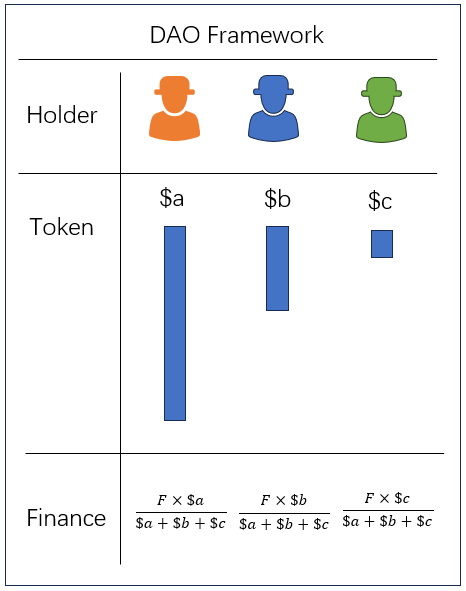
\includegraphics[width=3.2in]{assets/finance.png}
  \caption{Distribute Finance by Tokens}
  \label{fig:frameworkoffinance}
\end{figure}

In the DAO framework, as illustrated in Figure \ref{fig:frameworkoffinance}, token allocation follows a process where all participants, including authors, reviewers, readers, and publishers, are assigned contributions represented by tokens. This allocation is carried out based on the established procedures within the framework.
Within this context, Non-Fungible Tokens (NFTs) can be utilized as a means to determine the distribution proportions of tokens. NFTs are unique tokens that represent specific assets or contributions \cite{10034436}. By employing NFTs, the token allocation process becomes more granular, allowing for a more precise distribution based on the individual contributions of each participant.
When finance is generated within the framework, it is distributed among all token holders according to the predetermined token allocation mechanism. The allocation is determined by the proportion of tokens held by each participant, reflecting their respective contributions and responsibilities within the framework.
By implementing token allocation based on NFTs and distributing finance according to the token distribution mechanism, all stakeholders in the DAO framework receive their fair shares in proportion to their token holdings. This incentivizes active participation and ensures that contributors are rewarded appropriately for their contributions within the framework.
% DAO中的token分配如图2所示,参与框架的所有角色,如作者、审稿人、读者,再加上出版商,会按照流程进行贡献分配,贡献的用token来表示。此时,按照NFT的方式,把token作为分配的比例,一旦框架中产生了finance,就会按照token的分配方式进行分配,发放给所有holder。


\subsection{The Operation Process}
% 1页
% 介绍Journal DAO框架中参与者的各类角色,Journal DAO运行流程和实现的功能,以及token和finance如何流转。

In the practical implementation of the Journal DAO, this paper leveraged the Aragon framework to establish a decentralized and transparent infrastructure for academic publishing. The execution of the DAO involved several key steps to ensure a seamless and fair distribution of tokens among participants \cite{el2020overview}.
In a DAO, the concept of incentive mechanisms plays a crucial role in driving active participation and contributions. These mechanisms are designed to provide incentives and rewards to individuals or entities involved in the DAO's activities. By offering tangible benefits such as token rewards, governance rights, or recognition, participants are motivated to actively engage and contribute to the DAO's growth and development. Effective incentive mechanisms foster collaboration, maintain long-term motivation, and encourage innovation within the DAO community. The incentive design of journal dao promotes collaboration, maintains long-term incentives, and promotes innovation within the DAO community in the following aspects.
%在期刊 DAO 的实际实施中,我们利用 Aragon 框架建立了一个去中心化和透明的学术出版基础设施。 DAO 的执行涉及几个关键步骤,以确保代币在参与者之间的无缝和公正分配。
%在 DAO 中,激励机制的概念在推动积极参与和贡献方面发挥着至关重要的作用。这些机制旨在为参与 DAO 活动的个人或实体提供激励和奖励。通过提供代币奖励、治理权或认可等有形利益,参与者会被激励积极参与 DAO 的成长和发展并为其做出贡献。journal dao的激励设计在以下几个方面促进了协作、维护长期激励和促进DAO社区内的创新。

\begin{enumerate}
  \item Author Rewards:
  %作者奖励:

  Authors receive tokens based on the evaluation provided by reviewers during the submission process. The more constructive and impactful the reviews, the higher the token allocation to the authors.
  %作者根据评审人在提交过程中提供的评估获得代币。评审越有建设性和有影响力,作者获得的代币就越多。

  \item Reviewer Incentives:
  %评审者激励:
  
  Reviewers are rewarded with tokens for their valuable contribution to the peer-review process. This includes providing insightful feedback and assisting in maintaining the quality of published work.
  %评审者因其对同行评审过程的宝贵贡献而获得代币。这包括提供有深度的反馈和帮助维护已发布作品的质量。
  
  \item Publication and Download Rewards:
  %出版和下载奖励:
  
  Upon successful publication, both authors and users who download the papers are granted tokens. This encourages not only the creation of quality content but also its dissemination and accessibility.
  %在成功发布后,作者和下载论文的用户都会获得代币。这不仅鼓励了高质量内容的创作,还促进了其传播和获取。

  \item Citation Bonuses:
  %引用奖金:

  Authors receive additional tokens when their published work is cited by other researchers. This incentivizes the production of influential and impactful research that contributes to the academic community.
  %当其他研究人员引用作者已发布的作品时,作者将额外获得代币。这鼓励了产生有影响力和影响力研究的创作。

\end{enumerate}

\begin{figure}[h]
  \centering
  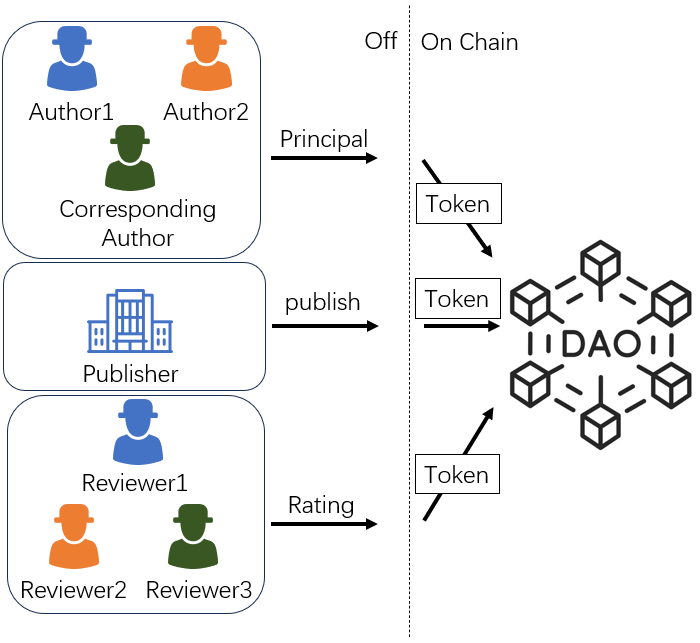
\includegraphics[width=3.2in]{assets/publishtoken.png}
  \caption{Distribute Token by DAO When Publishing}
  \label{fig:publishtoken}
\end{figure}


The workflow of the DAO, as shown in Figure \ref{fig:publishtoken} depicted in the diagram begins with the submission of a manuscript by the user for publication. As the DAO initiates the token minting process, specific rules guide the allocation of tokens. Authors are categorized into corresponding roles such as corresponding author, first author, second author, and third author, and so on, each receiving a different token allocation based on their contributions and responsibilities within the manuscript. Similarly, reviewers play a crucial role in the token allocation process. Their allocation is determined by their role in the review process and the ratings they provide for the submitted manuscripts. The publisher, as the platform responsible for facilitating manuscript publication, also receives a certain allocation of tokens due to their administrative role in managing the manuscripts. 

This meticulous token allocation mechanism ensures that each contributor, be it an author or a reviewer, receives fair rewards based on their specific contributions and responsibilities \cite{10123021}. By implementing such a structured system, the DAO creates a transparent and equitable environment, aligning the incentives for authors and reviewers. This not only cultivates a sense of fairness within the system but also encourages active and meaningful participation from all parties. Guided by DAO principles, the workflow fosters seamless integration of all stakeholders, ensuring a well-functioning and self-sustaining ecosystem.
%在图示的工作流程中,流程始于用户提交论文进行出版。随着DAO启动铸币过程,特定规则指导着代币的分配。作者根据其在论文中的角色分为通讯作者、第一作者、第二作者和第三作者,每个人按照贡献和责任都获得不同的代币分配。同时,审稿人在代币分配中发挥着至关重要的作用。他们的分配由他们在审稿过程中的角色和对提交的论文的评分决定。出版商作为提供论文发布的平台,又有管理论文的职责,也分配了一定的代币。这种细致入微的代币分配机制确保了每个贡献者,无论是作者还是审稿人,都能根据其具体的贡献和责任公正获得奖励。通过实施这样一个结构化的系统,DAO创造了一个透明而公平的环境,使作者和审稿人的激励保持一致。这不仅在系统内部培养了公正感,还鼓励各方积极而有意义地参与。受DAO原则指导的工作流程促进了各利益相关方的无缝整合,确保了一个运行良好且自我维持的生态系统。



\begin{figure}[h!]
  \centering
  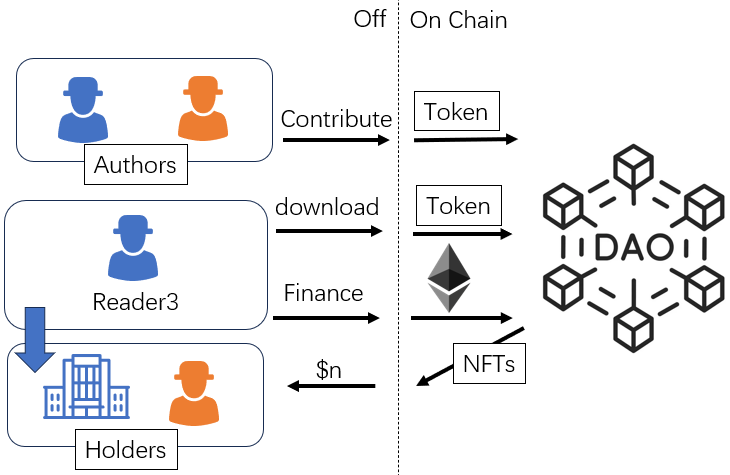
\includegraphics[width=3.2in]{assets/downloadfinance.png}
  \caption{Distribute Token and Dinance by DAO When Downloading}
  \label{fig:downloadfinance}
\end{figure}


In this system, authors, reviewers, publisher, readers(who download the papers or references) all possess a specific quantity of tokens. These tokens are considered as NFTs due to their unique nature. Once finance is generated, such as when a user pays to download a paper as Figure \ref{fig:downloadfinance}, the system allocates this finance based on the number of tokens held by the respective parties.This design ensures objectivity, fairness, and transparency within the system. Each participant's contribution is reflected in a specific number of tokens, and the allocation mechanism operates according to the quantity of these tokens. Such a design not only enhances the fairness of the incentive mechanism but also makes the entire system more transparent, allowing participants to clearly understand the relationship between their contributions and rewards.This NFT-based token system provides tangible and verifiable returns for contributors while establishing an effective and operable incentive mechanism for the entire ecosystem \cite{kong2021alternative}. This fair and transparent allocation method is expected to drive collaboration and development in the academic community, creating a mutually beneficial environment for all stakeholders.

%在这个系统中,作者、审稿人、下载用户和引用用户都拥有一定数量的token。这些token具有唯一性,可以被视为NFT(非同质化代币)。一旦产生了finance,比如用户通过付费下载论文,系统会按照持有者的token数量来分配这部分finance。这个设计确保了系统的客观性、公正性和透明性。每个参与者的贡献都以特定数量的token体现,而分配机制则按照这些token的数量来进行。这样的设计不仅提高了激励机制的公正性,也使得整个系统更加透明,参与者可以清晰地了解他们的贡献与奖励之间的关系。这种以NFT为基础的token系统为贡献者提供了具体的、可证明的回报,同时也为整个生态系统提供了一种有效的、可操作的激励机制。这种公正而透明的分配方式有望推动学术界的合作与发展,为各方创造一个共赢的环境。



\subsection{Advantages of Finance in Journal DAO}


In the current web2.0 landscape, both literature storage and payment systems are typically centralized, controlled by a single entity or organization. However, in the decentralized web3.0 network, article data resides directly on the blockchain \cite{alabdulwahhab2018web}, with websites serving as interfaces to access this data \cite{10402553}. 
In this new framework, payments for article downloads are automated and executed through smart contracts within the DAO framework \cite{cao2022decentralized}. This ensures complete transparency and traceability, as the fund distribution process follows predefined rules without centralized supervision \cite{10302676}. 


In the Web 3.0 paradigm, this novel model signifies a departure from reliance on traditional intermediaries. Instead, it empowers users with the direct participation in DAO frameworks, utilizing smart contracts for automated and secure fund distribution \cite{10302435}. This shift not only achieves decentralization in the transaction process but also enhances the efficiency of academic article transactions.
In the Web 3.0 environment, articles are directly uploaded to the blockchain. All operations, including payment processing and fund distribution, are seamlessly executed through smart contracts. This innovative framework ensures complete transparency and traceability throughout the entire process. When users pay to download articles, the funds are automatically allocated according to the rules established within the DAO framework, eliminating the need for any centralized oversight.
% 在当今web2.0的下,无论文献的储存或者支付系统,通常都是集中式的,这意味着它们由单个实体或组织控制。在去中心化网络的web3.0,文章数据主体直接存在于区块链上,而网站仅仅是对区块链数据的映射。在这一新的框架下,用户支付下载后,整个资金分配的过程都通过智能合约进行自动化执行,无需手动干预。这一创新性框架确保了整个过程的完全透明性和可追溯性。当用户支付下载文章时,资金会根据去中心化自治组织(DAO)框架内设立的规则自动分配,无需任何集中监管。
%在Web 3.0的范式中,这一新兴模式标志着我们不再依赖传统中介机构。相反,它赋予用户直接参与DAO框架的权力,利用智能合约实现资金的自动化和安全分配。这一转变不仅实现了交易过程的去中心化,还提高了学术文章交易的效率。
%在Web 3.0的环境中,文章直接上链。所有操作,包括支付处理和资金分配,都通过智能合约无缝执行。这一创新性框架确保了整个过程的完全透明性和可追溯性。当用户支付下载文章时,资金会根据去中心化自治组织(DAO)框架内设立的规则自动分配,无需任何集中监管。
  
\section{Mechanism Design of Journal DAO \label{sec:mechanism}}
% \section{Mechanism Design of Journal DAO \label{sec:mechanism}}本节共2页
% 简要写一下本节的思路,3-5行即可。

% \subsection{Decentralized Governance}

% \subsection{Initial Token Distributions}

% \subsection{Token Distributions upon Article Download or Citation}

% \subsection{Finance Distributions}




% 本文结合DAO的基本概念,创建DAO的框架。首先是铸币,其中为所有与论文相关的参与者,包括审稿人,作者,读者,按照一定的机制分配token。token可以用来决定proposal的权重,本框架根据token分配finance。
This paper combines the fundamental concepts of DAO to establish a framework for implementing DAO in academic journals. The framework begins with the issuance of tokens, which are allocated to all participants involved in the publication process, including reviewers, authors, and readers, through a specified mechanism. These tokens serve as a means to determine the weightage of proposals, and the framework utilizes the token distribution to allocate financial resources accordingly. By integrating token-based incentives and governance mechanisms, this framework ensures a fair and transparent distribution of resources within the DAO-operated journal ecosystem. Participants holding tokens can actively participate in the processes of all aspects of the article publication, such as send articles, review articles, and download articles, thereby influencing the allocation of financial resources based on their token holdings. Through this framework, the DAO-operated journal can foster an inclusive and democratic environment, empowering participants to shape the direction and priorities of the journal based on their token weightage.
%本文结合DAO的基本概念,创建了一个适用于学术期刊的DAO框架。该框架首先进行铸币操作,将与论文相关的所有参与者(包括审稿人、作者和读者)按照一定的机制分配代币。这些代币可以用来决定提案的权重,本框架则根据代币分配财务资源。通过整合代币激励和治理机制,该框架确保在DAO运营的学术期刊生态系统中资源的公平和透明分配。持有代币的参与者可以积极参与文章发布过程,例如发布文章、审阅文章和下载文章,从而根据其代币持有量影响财务资源的分配。通过该框架,DAO运营的学术期刊能够营造一个包容和民主的环境,赋予参与者根据其代币权重来塑造期刊的方向和优先事项的权力。


\begin{equation}
  \begin{bmatrix}
    A_t \\
    E_t \\
    P_t \\
    R_t 
  \end{bmatrix}
  = 
  \omega_{t-1}
  \begin{bmatrix}
    A_{t-1} \\
    E_{t-1} \\
    P_{t-1} \\
    R_{t-1}
  \end{bmatrix}
  +
  \omega_{t-2}
  \begin{bmatrix}
    A_{t-2} \\
    E_{t-2} \\
    p_{t-2} \\
    R_{t-2}
  \end{bmatrix}
  +
  \cdot
  + 
  \omega_n
  \begin{bmatrix}
    A_n \\
    E_n \\
    P_n \\
    R_n
  \end{bmatrix}
  \label{eq:dao}
\end{equation}



By applying the DAO framework to academic journals in accordance with the proposed Equation \ref{eq:dao}, each action taken within the system has the potential to alter future benefits. Through a well-structured incentive mechanism, the entire DAO ecosystem can achieve a state of perfect autonomy. This means that the actions and decisions made by participants, including authors, reviewers, and readers, have a direct impact on the overall functioning and success of the journal \cite{10426804}. With the right incentives in place, the DAO-operated journal can foster a self-sustaining and self-regulating environment, where participants are motivated to actively engage, contribute their expertise, and collectively drive the advancement of scholarly knowledge.
% 通过根据提议的方程 \ref{eq:dao} 将 DAO 框架应用于学术期刊,系统内采取的每项行动都有可能改变未来的效益。通过结构良好的激励机制,整个DAO生态系统可以达到完美自治的状态。这意味着包括作者、审稿人和读者在内的参与者的行动和决定对期刊的整体运作和成功有直接影响。通过适当的激励措施,DAO 运营的期刊可以营造一个自我维持和自我调节的环境,激励参与者积极参与、贡献他们的专业知识,并共同推动学术知识的进步。



\subsection{Decentralized Governance}
%去中心化治理:

DAO, adopting a decentralized governance model, allows token holders to participate in the decision-making process. This ensures community involvement in platform development, creating a democratic and inclusive environment. With robust incentives in place, token holders have made outstanding contributions while also receiving greater rewards. This positive feedback loop forms a self-sustaining ecosystem of active governance \cite{beck2018governance}. DAOs leverage blockchain technology to provide transparency and trust, recording all proposals, votes, and transactions on the blockchain for public verification. Incentives motivate token holders to actively engage in the governance process, while DAOs offer a meritocratic approach that values expertise. The flexibility and adaptability of DAOs allow them to evolve and respond to the needs of the community. However, challenges such as active participation, governance gridlocks, and power concentration need to be addressed through clear rules and mechanisms. Overall, DAOs empower token holders, foster community involvement, and create a democratic and inclusive environment.
%DAO采用去中心化治理模型,允许代币持有者参与决策过程。这确保了社区能够参与平台发展,创造了一个民主和包容的环境。在比较优秀的激励下,代币持有者做了出色的贡献,同时也获得更多的奖励。一个积极的自治体系完美闭环。DAO借助区块链技术提供透明度和信任度,将所有提案、投票和交易记录在区块链上,供公众验证。激励机制激励代币持有者积极参与治理过程,而DAO则提供了重视专业知识的优秀人才的机会。DAO的灵活性和适应性使其能够随着社区的需求而发展和应对变化。然而,需要通过明确的规则和机制来解决积极参与、治理僵局和权力集中等挑战。总体而言,DAO赋予代币持有者权力,促进社区参与,并创造民主和包容的环境。

\begin{figure}[ht]
  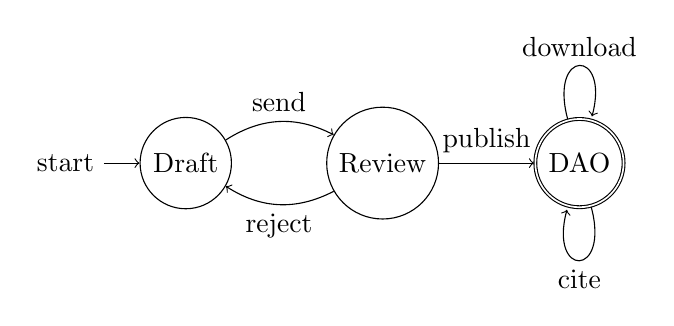
\begin{tikzpicture}[node distance=2.5cm, on grid]
    \node[state, initial] (q1) {Draft};
    \node[state, right=of q1] (q2) {Review};
    \node[state, accepting, right=of q2] (q3) {DAO};
  
    \path[->]
        (q1) edge[bend left, above] node {send} (q2)
        (q2) edge[bend left, below] node {reject} (q1)
        (q2) edge[left, above] node {publish} (q3)
        (q3) edge[loop above] node {download} (q3)
        (q3) edge[loop below] node {cite} (q3);
  \end{tikzpicture}
  \caption{Events of Article in Framework}
  \label{fig:decentralized_governance}
\end{figure}


The implementation of the Journal DAO (Figure \ref{fig:decentralized_governance}) has yielded positive results in terms of increased engagement, quality submissions, and a more inclusive academic ecosystem. The transparent and automated token distribution mechanisms have effectively addressed issues of ownership and reward distribution, fostering a collaborative and fair scholarly environment.
In order to create a strong incentive for active participation, a well-designed incentive mechanism is implemented in the decentralized governance framework. After authors publish their papers, the generated finance from user downloads is distributed not only to the publishers but also to all the authors and reviewers, motivating authors to produce high-quality articles and encouraging more individuals to serve as reviewers.
To further enhance participation, readers who download the papers are also allocated a share of the revenue. This encourages more people to download the papers, leading to increased revenue for the DAO. As a result, all participants are incentivized to actively engage in the ecosystem, fostering a thriving and automatic academic community.
This incentive mechanism ensures that all contributors, including authors, reviewers, and readers, are fairly rewarded for their contributions. It creates a positive cycle where authors are motivated to produce quality work, reviewers are incentivized to provide valuable feedback, and readers are incentivized to access and support the academic content. Overall, this system promotes a healthy and autonomous academic ecosystem within the DAO framework.
%期刊 DAO 的实施在提高参与度、质量投稿以及创建更具包容性的学术生态方面取得了积极成果。透明和自动化的代币分配机制有效解决了所有权和奖励分配的问题,促进了合作和公正的学术环境。
% 是用一个比较好的激励机制,让所有参与者都能积极参与。作者发表论文之后,用户下载时创造的finance除了给出版商外,所有的作者以及审稿人都可以分得收益,会让作者更有写作优秀文章的动力;审稿人也会获得收益,会有更多的人愿意做审稿人。现在,给下载论文的读者也分配收益,会有更多的人愿意下载论文,有更多的人下载论文,DAO就会有更多收益,这样就能让所有的参与者都能积极参与,形成一个良好的自治学术生态。

\subsection{Initial Token Distributions}

In the DAO framework, tokens are minted during key events such as article publication, downloads, and citations, and then distributed to participants according to predetermined proportions. All these processes are executed through smart contracts, ensuring transparency and traceability. Having a well-designed token allocation mechanism forms the foundation of the entire framework, enabling a self-sustaining and self-regulating environment.
With a fair token distribution mechanism, the DAO framework can create a system where participants are incentivized to contribute and engage actively. The allocation of tokens based on specific events fosters a sense of fairness and encourages collaboration among authors, readers, reviewers, and publishers. The transparent and traceable nature of the smart contract-based processes ensures that the token distribution is open to scrutiny and can be verified by all participants.
In this self-regulating environment, the DAO framework can adapt and adjust dynamically based on the actions and contributions of its participants. The token allocation mechanism serves as a means to reward and recognize the efforts of contributors, fostering a sustainable ecosystem where knowledge sharing and collaboration thrive.
% DAO框架在关键的事件进行铸币,如文章的发布,被下载,被引用,然后按照一定比例将其分发给各个参与者。所有过程经过智能合约完成,保证透明以及可追溯。有了合理的token分配机制,是整个框架的基础,可以实现自我维护和自我调节的环境。

\begin{equation}
  \begin{aligned}
    D_0 &= \sum_{i = 1}^{m}x_i \\
    1 &= \alpha_1 + \alpha_2 + \alpha_3 \\
    A_0 &= \alpha_1 D_0 \quad (A=\{a_0, a_1, a_2, a_3, \cdots a_n\}) \\
    E_0 &= \alpha_2 D_0 \quad (E=\{e_1, e_2, e_3, \cdots e_m\}) \\
    P_0 &= \alpha_3 D_0 \quad (P=\{p\})
  \end{aligned}
  \label{eq:dao0}
\end{equation}

Upon publication of an article, a DAO specific to that particular article is established, and tokens are minted and distributed among the authors, reviewers, and the publisher. The total number of tokens minted after this process, denoted as $D_0$, is determined based on Equation \ref{eq:dao0}, taking into account the distribution proportions among the three parties: $\alpha_1$, $\alpha_2$, and $\alpha_3$. Consequently, the allocation of tokens is as follows: the authors receive $A_0 = \alpha_1 D_0$, the reviewers receive $E_0 = \alpha_2 D_0$, and the publisher receives $P_0 = \alpha_3 D_0$.
%文章发表时候,创建一个当前article的DAO,铸币分给作者,审稿人和出版商。根据公式\ref{eq:dao0}$D_0$为本次铸币之后的总token数量,三方占比为$\alpha_1$,$\alpha_2$和$\alpha_3$。则作者分到$A_0 = \alpha_1 D_0 $,审稿人分到$E_0 = \alpha_2 D_0 $,出版商分到$P_0 = \alpha_3 D_0 $


\begin{equation}
  \begin{aligned}
    1 &= \beta_0 + \beta_1 + \beta_2 + \beta_3 + \cdots + \beta_n (\beta_1 \geq  \beta_2 \geq \beta_3 \cdots \geq \beta_n)\\
    a_{i} &= \beta_i A \quad (a \in A) \\
    a_{i0} &= \beta_i A_0 \quad (a_0 \in A_0 )
  \end{aligned}
  \label{eq:authorrate}
\end{equation}

In the case of having a total of $n$ authors, the allocation of tokens for each author is determined by the proportions specified in Equation \ref{eq:authorrate}. In this equation, $\beta_0$ represents the token allocation for the corresponding author, $\beta_1$ represents the token allocation for the first author, $\beta_2$ represents the token allocation for the second author, and so on. The total number of tokens allocated to all authors is denoted as $A$, and each author $a_i$ receives a portion of tokens distributed according to the respective $\beta$ ratio.When the article is published, tokens are minted and distributed to all authors. The total number of tokens allocated to the authors is denoted as $A_0$, and each author $a_{i0}$ receives tokens distributed in the same proportions as determined by the $\beta$ ratios.
%作者数量为n,每个作者分到的的token数量占比见公式\ref{eq:authorrate},其中$\beta_0$特指为通讯作者,$\beta_1$为一作,$\beta_2$为二作,以此类推。所有作者的token为$A$,每个作者$a_i$的token按照$\beta$比例分配。文章法布时,铸币给所有作者的token数量为$A_0$,每个作者$a_i0$按照同样的比例分配。

\begin{equation}
  \begin{aligned}
    1 &= \gamma_1 + \gamma_2 + \gamma_3 + \cdots + \gamma_m \\
    e_{i} &= \gamma_i E \quad (e \in E) \\
    e_{i0} &= \gamma_i E_0 \quad (e_0 \in E_0 )
  \end{aligned}
  \label{eq:reviewerrate}
\end{equation}

The number of reviewers is denoted as $m$, the allocation of tokens for each reviewer follows the proportions specified in Equation \ref{eq:reviewerrate}. In this equation, the token allocation for each reviewer $e_i$ is determined by the respective $\gamma$ ratio. The proportions for the reviewers may be determined based on other factors, such as the role the reviewers. The total number of tokens allocated to all reviewers is denoted as $E$.When the article is published, tokens are minted and distributed to all reviewers. The total number of tokens allocated to the reviewers is denoted as $E_0$, and each reviewer $e_{i0}$ receives tokens distributed in the same proportions as determined by the $\gamma$ ratios. The distribution mechanism remains consistent with that of the authors.
%审稿人数量为m,每个审稿审稿人分到的token数量占比见公式\ref{eq:reviewerrate},审稿人分得的比例按照其他方式决定,如角色定位。与作者相同,所有审稿人的token为$E$,每个审稿人$e_i$的token按照$\gamma$比例分配。文章法布时的铸币分配方式与之前相同,所有审稿人的token数量为$E_0$,每个审稿人$e_i0$按照$\gamma$比例分配。

\subsection{Token Distributions upon Article Download or Citation}

Unlike the singular issuance of tokens associated with article publication, the act of downloading articles by users as readers is a recurring event that perpetually exists within the DAO framework. The act of downloading an article not only represents recognition of the article itself but also serves as recognition of the article's author. Therefore, tokens need to be allocated to the authors, with the primary author and corresponding author, who contribute the most, receiving a larger share.
Furthermore, readers who download articles both recognize the value of the article and also receive tokens as a result. This dual recognition mechanism ensures that both authors and readers are rewarded within the DAO framework. By allocating tokens to authors and readers, the system fosters a sense of acknowledgment and incentivizes active participation from all stakeholders involved in the publication and consumption of articles.
% 区别于文章法布的唯一铸币,用户作为读者阅读文章之后的下载,是一个多次事件,永远存在于DAO框架中。文章被下载,代表了对文章的认可,更是对文章作者的认可,所以token需要分给作者,贡献最大的一作和通讯作者获得更多。读者作为下载文章的用户,认可了文章同样也获得了token。

\begin{equation}
  \begin{aligned}
    D_1 &= D_{1a} + D_{1r} \\
    A_1 &= D_{1a} \\
    \Sigma^A_1 &= A_0 + A_1 \\
    E_1 &= 0 \\
    P_1 &= 0 \\
    R_1 &= D_{1r} \\
  \end{aligned}
  \label{eq:downloadtoken}
\end{equation}

After the publication of the article, when users read and download the article, additional token minting occurs according to the formula specified in Equation \ref{eq:downloadtoken}. The purpose of this additional token minting is to incentivize authors and provide benefits to readers. In this process, new tokens are allocated to both authors and readers, while the token allocations for reviewers and the publisher remain unchanged.
% 文章发布之后,有用户阅读并下载了文章,此时会继续铸币,见公式\ref{eq:downloadtoken}。为了鼓励作者,以及让利给读者,新的token分给作者以及读者,审稿人以及出版商的token保持不变。

\begin{equation}
  \begin{aligned}
    1 &= \beta_{1, 0} + \beta_{1, 1} + \beta_{1, 2} \\
    a_{1,0} &= A_1 \beta_{1, 0}  \\
    a_{1,1} &= A_1 \beta_{1, 1}  \\
    a_{1,2} &= A_1 \beta_{1, 2}  \\
  \end{aligned}
  \label{eq:downloadrate}
\end{equation}

According to Equation \ref{eq:downloadrate}, the tokens generated through the user's download behavior will be allocated to the corresponding author, first author, and second author in certain proportions. However, the token allocations for other authors remain unchanged.
% 根据公式\ref{eq:downloadrate},用户下载行为时铸币生成的token,会按照一定的比例分给通讯作者,一作以及二作,其他作者的token保持不变。


\begin{equation}
  \begin{aligned}
    D_2 &= D_{2a} + D_{2r} \\
    A_2 &= D_{2a} \\
    \Sigma^A_2 &= A_0 + A_1 + A_2 \\
    E_2 &= 0 \\
    P_2 &= 0 \\
    R_2 &= D_{2r} \\
    \Sigma_{r1} & = R_1 + R_2 \quad if \quad R_1 = R_2 \quad (r_1 \in R ) 
  \end{aligned}
  \label{eq:citetoken}
\end{equation}

According to Equation \ref{eq:citetoken}, if a user cites a previously downloaded article in their own article, it triggers token minting. The tokens generated in this case are allocated to both the authors of the cited article and the user who made the citation.
% 根据公式\ref{eq:citetoken},用户自己发了论文引用了之前下载的论文,也会出发铸币,token同样分给作者以及引用的用户。



\subsection{Finance Distributions by Token}

By employing token allocation based on NFT principles, the framework ensures a fair distribution of rewards among token holders. Through transparent smart contracts, the DAO framework establishes a self-regulating environment that incentivizes active participation and contribution. The implementation of this token-based distribution mechanism requires tracking token ownership and automated distribution of finance.
% 按照nft的方式,把token作为分配的比例,一旦产生了finance,就按照所有holder都可以按照比分到finance。

\begin{equation}
  \begin{aligned}
    1 &= \frac{A}{D} + \frac{E}{D} + \frac{P}{D} + \frac{R}{D} = \alpha_1 + \alpha_2 + \alpha_3 + \alpha_4 \\
    F &= finance \\
    F_A &= \alpha_1 F \quad (A=\{a_0, a_1, a_2, a_3, \cdots a_n\}) \\
    F_E &= \alpha_2 F \quad (E=\{e_1, e_2, e_3, \cdots e_m\}) \\
    F_P &= \alpha_3 F \quad (P=\{p\}) \\ 
    F_R &= \alpha_4 F \quad (R=\{r_1, r_2, r_3, \cdots r_i\})
  \end{aligned}
  \label{eq:finance}
\end{equation}


According to Equation \ref{eq:finance}, the token allocation ratios for authors, reviewers, publisher, and readers are denoted as $\alpha_1$, $\alpha_2$, $\alpha_3$, and $\alpha_4$, respectively. Once finance is generated, it is distributed to all token holders based on these ratios. 
To respect intellectual property rights, many publishers require users to pay for downloading articles. In such cases, finance enters the DAO and is distributed to all authors, reviewers, publisher, and readers according to their token ratios. Articles typically attract a significant number of downloads, with exceptional ones garnering even more. Importantly, this distribution mechanism enables sustained earnings, thereby incentivizing authors to produce higher quality articles. 
While users initially act as consumers when downloading articles, they also become partial owners of the downloaded articles. As a result, they are eligible to receive a portion of the generated finance based on their token ratios. Motivating readers is crucial as it encourages them to willingly pay for article downloads, ultimately creating more finance and fostering a real automated organization. 
By implementing this approach, all participants receive fair allocations for their contributions. The autonomous nature of the framework drives authors to produce outstanding articles and incentivizes readers to pay for downloads, thereby generating more finance and establishing a virtuous cycle within the system.
% 根据公式\ref{eq:finance},作者、审稿人、出版商、读者的token分配比例为$\alpha_1$, $\alpha_2$, $\alpha_3$, $\alpha_4$,一旦产生finance,会按照这个比例分给所有holder。比如为了尊重知识产权,很多出版商的论文需要用户付费下载,此时就有了finance进入DAO,并按照token的比例分给了所有作者、审稿人、出版商、读者。文章的下载量一般会很多,优秀的文章下载量更多,最重要的是可以持续收益,这种情况下,激励了作者写出更优秀的article。用户作为读者下载文章本是消费者,但是下载文章之后既变成文章的拥有者之一,之后的finance也会分给这个读者。对读者的激励十分重要,这让读者更愿意付费下载article,也就创造了更多的finance,形成一个完美的自治。






\section{A Case Study \label{sec:performance}}


\begin{table*}[ht!]
  \begin{center}
    \caption{Finance for DAO.}
    \label{tab:finance}
    \begin{tabular}{r|l|l|l|l|l|l|l|l|l} % <-- Alignments: 1st column left, 2nd middle and 3rd right, with vertical lines in between
      & \multicolumn{4}{c|}{\textbf{Authors}} & \textbf{Publisher} & \multicolumn{2}{c|}{\textbf{Reviewers}} & \multicolumn{2}{c}{\textbf{Readers}}\\
      \hline
      \textbf{index} & \textbf{Corresponding} & \textbf{Author1} & \textbf{Author2} & \textbf{Author3} & \textbf{Publisher} & \textbf{Reviewer1} & \textbf{Reviewer2} & \textbf{Download} & \textbf{Cite}\\
      \hline
      0 & 0.122997 & 0.184696 & 0.061298 & 0.030449 & 0.200321 & 0.177885 & 0.222356 & 0 & 0 \\
      1 & 0.124113 & 0.186367 & 0.061860 & 0.029945 & 0.197006 & 0.174941 & 0.218676 & 0.007092 & 0 \\
      2 & 0.125194 & 0.187984 & 0.062403 & 0.029457 & 0.193798 & 0.172093 & 0.215116 & 0.006977 & 0 \\
      3 & 0.125000 & 0.187688 & 0.062312 & 0.028529 & 0.187688 & 0.166667 & 0.208333 & 0.006757 & 0.013514 \\
      4 & 0.126016 & 0.189209 & 0.062823 & 0.028086 & 0.184775 & 0.164080 & 0.205100 & 0.006652 & 0.013304 \\
      5 & 0.127001 & 0.190684 & 0.063319 & 0.027656 & 0.181951 & 0.161572 & 0.201965 & 0.006550 & 0.013100 \\
      6 & 0.127957 & 0.192115 & 0.063799 & 0.027240 & 0.179211 & 0.159140 & 0.198925 & 0.006452 & 0.012903 \\
      7 & 0.128884 & 0.193503 & 0.064266 & 0.026836 & 0.176554 & 0.156780 & 0.195975 & 0.006356 & 0.012712 \\
      8 & 0.129784 & 0.194850 & 0.064718 & 0.026444 & 0.173974 & 0.154489 & 0.193111 & 0.006263 & 0.012526 \\
      9 & 0.130658 & 0.196159 & 0.065158 & 0.026063 & 0.171468 & 0.152263 & 0.190329 & 0.006173 & 0.012346 \\
      10 & 0.131508 & 0.197431 & 0.065585 & 0.025693 & 0.169033 & 0.150101 & 0.187627 & 0.006085 & 0.012170 \\
      11 & 0.132333 & 0.198667 & 0.066000 & 0.025333 & 0.166667 & 0.148000 & 0.185000 & 0.006000 & 0.012000 \\
      12 & 0.133136 & 0.199869 & 0.066404 & 0.024984 & 0.164366 & 0.145957 & 0.182446 & 0.005917 & 0.011834 \\
      13 & 0.133917 & 0.201038 & 0.066796 & 0.024643 & 0.162127 & 0.143969 & 0.179961 & 0.005837 & 0.011673 \\
      14 & 0.134677 & 0.202175 & 0.067179 & 0.024312 & 0.159949 & 0.142035 & 0.177543 & 0.005758 & 0.011516 \\
      15 & 0.134268 & 0.201558 & 0.066978 & 0.023676 & 0.155763 & 0.138318 & 0.172897 & 0.005607 & 0.011215 \\
      16 & 0.134994 & 0.202645 & 0.067343 & 0.023370 & 0.153752 & 0.136531 & 0.170664 & 0.005535 & 0.011070 \\
      17 & 0.135701 & 0.203704 & 0.067699 & 0.023072 & 0.151791 & 0.134791 & 0.168488 & 0.005464 & 0.010929 \\
      18 & 0.136391 & 0.204736 & 0.068046 & 0.022782 & 0.149880 & 0.133094 & 0.166367 & 0.005396 & 0.010791 \\
      19 & 0.137063 & 0.205743 & 0.068384 & 0.022499 & 0.148017 & 0.131439 & 0.164298 & 0.005329 & 0.010657 \\
      20 & 0.137719 & 0.206725 & 0.068713 & 0.022222 & 0.146199 & 0.129825 & 0.162281 & 0.005263 & 0.010526 \\
      Total & 2.749313 & 4.127544 & 1.371082 & 0.543292 & 3.574286 & 3.173966 & 3.967458 & 0.121463 & 0.214788 \\
    \end{tabular}
  \end{center}
\end{table*}



In addition to the theoretical framework, there need conducted simulations to evaluate the effectiveness of the proposed DAO system \cite{macal2009agent}. Table \ref{tab:finance} presents results from 20 simulated downloads, illustrating the distribution of finance among holders. This simulation provides a comprehensive overview of how finance is allocated to holders based on their token holdings \cite{liu2023incremental}.
Within the DAO framework, authors, as the owners of the articles, experience an increase in their tokens and ownership ratio when their articles are downloaded or cited, leading to higher profits. Reviewers, as participants in the article review process, initially receive tokens that do not increase over time. Although their ownership ratio gradually decreases, their profits continue to increase. The accuracy of their ratings directly benefits themselves. Readers, during the process of downloading and citing, also receive tokens, albeit in smaller quantities and with lower ownership ratios. However, as the articles are downloaded or cited, their overall profits increase. Additionally, the profit margin gradually decreases, meaning that readers who download and cite the articles in the early stages will benefit from higher profits, thus incentivizing the early identification of outstanding articles.
%在论文中,我们不仅提出了理论框架,还进行了模拟实验来评估提出的DAO系统的有效性。表格1展示了20次模拟下载的结果,说明了finance在持有者之间的分配情况。这个模拟提供了一个全面的概述,说明了根据令牌持有情况如何分配finance。
% 在这个dao框架之下,author作为文章的拥有者,在文章被下载或被引用时,其token会增加,并且占有率也在增加,同时收益就会越来越高。reviewer作为文章的参与者,他们初期会收到相应的token,但是不再增加,虽然占比逐渐降低,但是收益总是是增加的,评分越准,对自己越有利。reader在download以及cite过程中,都会收到相应的token,虽然量少,并且占有率也不高,但是随着文章被下载或被引用,总收益就也会越来越高。并且在这个过程中,收益率是逐渐下降的,也就是在论文早期下载和引用的reader,会活动比较高的收益,这鼓励了早期识别优秀的论文。


\subsection{Proportion of Trend}


\begin{figure}[h]
  \centering
  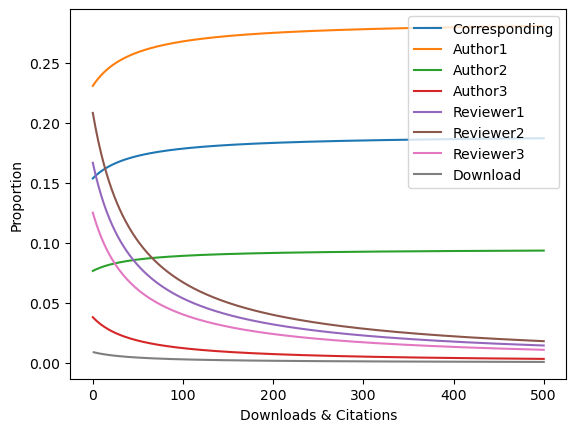
\includegraphics[width=3.2in]{assets/proportion-all.png}
  \caption{Proportion of All.}
  \label{fig:proportion-all}
\end{figure}

Integrating DAO technology into the realm of academic journals holds immense potential for benefiting authors, reviewers, and readers alike. Look at Figure \ref{fig:proportion-all}.
Authors, being the rightful owners of their published works, would reap the most substantial rewards from such a system. By leveraging the decentralized nature of DAOs, authors can secure a greater share of the financial gains associated with their articles. As time progresses, their earnings could potentially increase, providing a long-term incentive for continued contributions.
Reviewers, as the gatekeepers and custodians of scholarly integrity, would also stand to gain from the implementation of DAOs in journals. Initially, they would hold a higher proportion of benefits, reflecting their crucial role in the early stages of article evaluation. However, as time progresses and articles are published, their share of benefits may gradually diminish, ensuring a fair distribution of rewards among all stakeholders.
Readers, as active participants in the scholarly discourse, would also have the opportunity to benefit from DAO-operated journals. While their gains may be comparatively lower than authors and reviewers, early engagement with the DAO ecosystem could yield higher returns. By accessing articles and participating in the DAO's governance processes, readers can contribute to the growth and success of the journal, potentially increasing their benefits over time.
The implementation of DAO mechanisms, such as token-based incentives, transparent governance structures, and decentralized decision-making processes, would enable a fair and equitable model for academic journals. This model fosters a sense of ownership, rewards active participation, and ensures the sustainability and long-term viability of the journal ecosystem.
%将 DAO 技术整合到学术期刊领域具有巨大的潜力,可以使作者、审稿人和读者受益
%作者作为其已发表作品的合法所有者,将从这样的系统中获得最丰厚的回报。通过利用 DAO 的去中心化性质,作者可以获得与其文章相关的更大份额的经济收益。随着时间的推移,他们的收入可能会增加,从而为持续贡献提供长期激励。
%审稿人作为学术诚信的看门人和守护者,也将从期刊中 DAO 的实施中获益。最初,他们将获得较高比例的收益,这反映了他们在文章评估的早期阶段的关键作用。然而,随着文章的发布,他们的利益份额可能会逐渐减少,从而确保所有利益相关者之间公平分配奖励。
%读者作为学术讨论的积极参与者,也将有机会从 DAO 运营的期刊中受益。虽然他们的收益可能相对低于作者和审稿人,但早期参与 DAO 生态系统可能会产生更高的回报。通过访问文章并参与 DAO 的治理流程,读者可以为期刊的发展和成功做出贡献,并有可能随着时间的推移增加其收益。
%DAO 机制的实施,例如基于代币的激励、透明的治理结构和去中心化的决策流程,将为学术期刊提供公平公正的模式。这种模式培养主人翁意识,奖励积极参与,并确保期刊生态系统的可持续性和长期生存能力。



\subsection{Break Even of User Download}

Indeed, allowing users to offset their expenses or even earn profits through downloading articles can effectively stimulate user participation. While individual reader earnings may be modest, readers constitute the largest group within the DAO framework, making them a critical factor for the system's autonomy.
By providing readers with the opportunity to offset their expenses or earn profits, the DAO framework can incentivize their active engagement. Despite individual earnings being relatively small, the cumulative impact of a large number of readers participating in the ecosystem contributes significantly to the overall success and sustainability of the DAO \cite{leimeister2010collective}. As a result, readers play a crucial role in driving the self-governing nature of the DAO framework.
% 用户作为读者下载文章,虽然需要付费,但是如果后面会收支相抵,甚至赚钱,会有效的刺激用户参与。虽然单个reader收益很少,但是在整个DAO框架中,数量最大,是DAO可以可以自治的核心因素。

\begin{figure}[h]
  \centering
  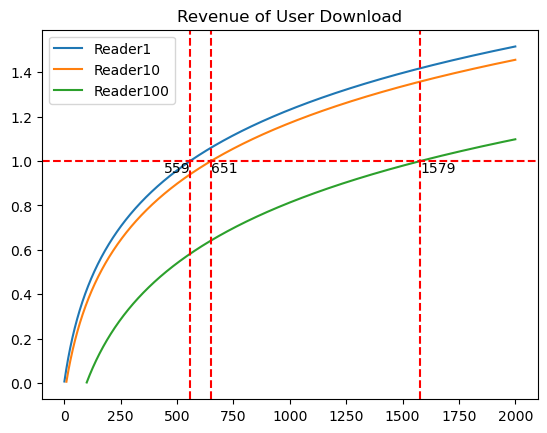
\includegraphics[width=3.2in]{assets/revenue-user-download.png}
  \caption{Revenue of User Download.}
  \label{fig:revenue-user-download}
\end{figure}

The total revenue for downloading users is depicted in Figure \ref{fig:revenue-user-download}. As readers who own the downloaded articles, their total revenue increases with a growing number of users downloading the articles. However, as more readers download the article and become owners, the individual token proportion naturally decreases. Consequently, the per-download revenue gradually declines.
To simulate the distribution ratios following scenario, mainly look at the key break-even points\cite{norreklit2000balance}: the first reader who downloads the article breaks even when the article is downloaded 559 times; the tenth reader breaks even when the article reaches 651 downloads; and the one hundredth reader breaks even at a staggering 1579 downloads. This incentive mechanism aims to encourage readers to discover exceptional articles earlier rather than following the crowd since owning the article no longer yields significant returns.
This approach incentivizes readers to identify outstanding articles sooner, as the potential for substantial earnings diminishes once an article has already demonstrated its quality.
% 下载用户的总收益如图 \ref{fig:revenue-user-download} 所示,随着更多用户下载article,作为读者的article拥有者,总收益会越来越多,但是因为更多其他读者下载article也获取了token,成为了article的拥有者,自己token的占比势必会减少,所以单次收益逐渐降低。设定分配比例进行模拟,第一个下载论文的读者,在文章被下载559次时,总收入与下载时的支出持平;第十个下载论文的读者,收支相抵时候需要文章被下载651次;第一百个下载论文的读者,收支相抵更是要到1579次。此种激励方式在于,如果文章已经证明很优秀了,再拥有已经不能得到多少收益了,鼓励读者更早发现优秀的文章,而不是跟风。


\subsection{Real Article simulation}


\begin{table*}[t!]
  \begin{center}
    \caption{Finance of Real Article for DAO.}
    \label{tab:realpaper}
    \begin{tabular}{r|l|l|l|l|l|l|l|l|l} % <-- Alignments: 1st column left, 2nd middle and 3rd right, with vertical lines in between
      & \multicolumn{4}{c|}{\textbf{Authors}} & \textbf{Publisher} & \multicolumn{2}{c|}{\textbf{Reviewers}} & \multicolumn{2}{c}{\textbf{Readers}}\\
      \hline
      \textbf{index} & \textbf{Corresponding} & \textbf{Author1} & \textbf{Author2} & \textbf{Author3} & \textbf{Publisher} & \textbf{Reviewer1} & \textbf{Reviewer2} & \textbf{Download} & \textbf{Cite}\\
      \hline
      0 & 0.122997 & 0.184696 & 0.061298 & 0.030449 & 0.200321 & 0.177885 & 0.222356 & 0 & 0 \\
      1 & 0.124113 & 0.186367 & 0.061860 & 0.029945 & 0.197006 & 0.174941 & 0.218676 & 0.007092 & 0 \\
      2 & 0.125194 & 0.187984 & 0.062403 & 0.029457 & 0.193798 & 0.172093 & 0.215116 & 0.006977 & 0 \\
      3 & 0.126240 & 0.189550 & 0.062929 & 0.028986 & 0.190694 & 0.169336 & 0.211670 & 0.006865 & 0 \\
      4 & 0.127252 & 0.191066 & 0.063438 & 0.028529 & 0.187688 & 0.166667 & 0.208333 & 0.006757 & 0 \\
      ... & ... & ... & ... & ... & ... & ... & ... & ... & ... \\

      998 & 0.184995 & 0.277503 & 0.092486 & 0.001690 & 0.011121 & 0.009876 & 0.012345 & 0.000400 & 0.000801 \\
      999 & 0.185000 & 0.277511 & 0.092489 & 0.001689 & 0.011111 & 0.009867 & 0.012333 & 0.000400 & 0.000800 \\
      1000 & 0.185005 & 0.277519 & 0.092491 & 0.001687 & 0.011101 & 0.009857 & 0.012322 & 0.000400 & 0.000799 \\
      1001 & 0.185010 & 0.277526 & 0.092494 & 0.001686 & 0.011090 & 0.009848 & 0.012310 & 0.000399 & 0.000799 \\
      1002 & 0.185015 & 0.277534 & 0.092497 & 0.001684 & 0.011080 & 0.009839 & 0.012299 & 0.000399 & 0.000798 \\
      
      ... & ... & ... & ... & ... & ... & ... & ... & ... & ... \\

      2151 & 0.186032 & 0.279053 & 0.093011 & 0.000803 & 0.005285 & 0.004693 & 0.005867 & 0.000190 & 0.000381 \\
      2152 & 0.186034 & 0.279056 & 0.093012 & 0.000803 & 0.005283 & 0.004691 & 0.005864 & 0.000190 & 0.000380 \\
      2153 & 0.186036 & 0.279059 & 0.093013 & 0.000803 & 0.005281 & 0.004689 & 0.005861 & 0.000190 & 0.000380 \\
      2154 & 0.186038 & 0.279062 & 0.093014 & 0.000802 & 0.005278 & 0.004687 & 0.005859 & 0.000190 & 0.000380 \\
      Total & 392.406327 & 588.652390 & 196.160264 & 6.520750 & 42.899672 & 38.094909 & 47.618636 & 1.537177 & 1.768627 \\
      
    \end{tabular}
  \end{center}
\end{table*}

Furthermore, we applied our DAO framework to a real-world case by analyzing a published paper with 2154 downloads and 42 citations. As shown in Table \ref{tab:realpaper}. By simulating the income distribution within the current DAO structure, we observed that download users not only offset their initial payment but also gained additional earnings. The incentivized system encourages users to respect copyright and, more importantly, has achieved a level of autonomy.The provided tables and case study demonstrate the practical application and positive outcomes of our proposed DAO framework. By aligning incentives with user behaviors, the system not only offsets costs for downloaders but also significantly incentivizes engagement. This not only respects copyright but also establishes a self-sustainable and autonomous ecosystem, providing valuable insights for the future development of decentralized academic publishing.

%此外,我们将DAO框架应用于一个真实案例,分析了一篇被下载2154次、引用42次的论文。通过模拟当前DAO结构下的收入分配情况,我们观察到下载用户不仅抵消了初始支付,还获得了额外的收益。这个激励系统鼓励用户尊重版权,更重要的是实现了一定程度的自治。提供的表格和案例研究展示了我们提出的DAO框架的实际应用和积极成果。通过将激励与用户行为保持一致,该系统不仅为下载者抵消了成本,还极大地激励了用户参与。这不仅尊重版权,还建立了一个自我可持续和自治的生态系统,为分散的学术出版的未来发展提供了有价值的见解。



After voluntarily making a payment, users' ability to participate contributes to a robust incentive mechanism, fostering a sense of autonomy within the entire framework. Through this design, users become direct contributors to financial activities, injecting new value into the framework and creating potential opportunities for self-reward. This decentralized autonomous model empowers users to engage directly in decision-making and contributions, shaping a more open, fair, and virtuous ecosystem. Overall, this autonomous framework cultivates a more positive and sustainable participation experience for users and the entire community.
Through the detailed simulations and analyses, the incentive mechanisms within the DAO framework emerge as crucial drivers in shaping the dynamics of authorship and user participation. As downloads and citations increase, the token-driven rewards become a powerful motivator for authors, leading to an accumulation of influence and financial gains. This incentive structure not only acknowledges and rewards the contributions of authors but also establishes a direct correlation between their efforts and the benefits they accrue.
Furthermore, users who engage with the system by downloading papers witness a direct impact on their influence and, subsequently, on their earnings. This creates a dual incentive structure, where authors and users are mutually motivated to contribute to and participate in the DAO environment. The concept of decentralized autonomy becomes evident as the system operates independently, fostering a self-sustaining loop of contributions, rewards, and governance.
In this context, the DAO framework provides a powerful tool for aligning interests and promoting a fair distribution of rewards based on tangible contributions. The transparency and automation inherent in DAO contribute to a governance model that minimizes external intervention, allowing the ecosystem to evolve organically through the collective actions of its participants. This synergy of incentives and autonomy within DAO not only enhances the overall efficiency of the academic publishing model but also creates a robust and self-regulating environment for authors and users alike \cite{ostrom1990governing}.
%用户自主付费后,其参与框架的能力构成了一种积极的激励机制,为整个系统的自治性提供了有力支持。通过这一设计,用户成为财务活动的直接贡献者,其行为不仅为框架注入了新的价值,同时也为自身创造了潜在的奖励机会。这种去中心化的自治模式使得用户能够更加直接地参与决策和贡献,从而塑造了一个更加开放、公正、而且具有良性循环的生态系统。整体而言,这种自治的框架为用户和整个社区创造了更为积极和可持续的参与体验。
%通过详尽的模拟和分析,DAO框架内的激励机制成为塑造作者和用户参与动态的关键推动因素。随着下载和引用的增加,基于代币的奖励变得越来越成为作者的强大动力,导致权重和财务收益的积累。这种激励结构不仅承认并奖励了作者的贡献,还在作者的努力和他们获得的收益之间建立了直接的关系。
%此外,通过下载论文积极参与系统的用户在他们的影响力和随之而来的收入上见证了直接的影响。这创建了一个双重的激励结构,使作者和用户相互激励,以在DAO环境中做出贡献和参与。去中心化自治的概念在系统自主运作中变得明显,形成了一个贡献、奖励和治理的自我维持循环。
%在这种情况下,DAO框架为协调利益和促进基于实际贡献的公平奖励分配提供了强大的工具。DAO内在的透明度和自动化有助于最小化外部干预的治理模型,通过参与者的集体行动,使生态系统有机地演变。DAO内的激励和自治的协同作用不仅提升了学术出版模型的整体效率,而且为作者和用户创造了一个强大而自我调节的环境。



% Once the paper is on the blockchain, it unequivocally belongs to the author, author is the real owner,that creating endless possibilities, especially in terms of financial activities. This means that the author not only owns their work but can also leverage blockchain technology to create various financial opportunities. Authors can receive rewards through financial activities, which may include paid downloads, knowledge exchanges, collaborative projects, and more. This decentralized framework provides authors with greater creative freedom and potential economic returns, enabling them to be more independent and influential in the academic domain. Overall, putting a paper on the blockchain opens up a new and forward-thinking path for authors.
% %论文一旦上链,将完全归属于作者,作者就是真正的拥有者,为作者创造了无限的可能性,特别是在财务活动方面。这意味着作者不仅拥有其作品的所有权,而且可以利用区块链技术创造各种财务机会。作者可以通过财务活动获得回报,这可能包括付费下载、知识交流、合作项目等。这种去中心化的框架为作者提供了更大的创作自由和潜在的经济回报,使其在学术领域更加独立和有影响力。整体而言,论文上链为作者开辟了一个全新的、具有前瞻性的创作道路。



\section{Conclusion \label{sec:conclusion}}
This paper extensively explores the framework of DAO and provides a thorough analysis of its potential applications in the academic publishing domain. By placing papers on the blockchain, we have achieved transparency in ownership, allowing authors to have complete control over their works while also creating diverse financial opportunities. The autonomous nature of DAO enables users to directly participate in decision-making and contributions, constructing an ecosystem that is open, fair, and characterized by positive feedback loops.
Under this framework, users can not only pay for paper downloads but also receive rewards through participation in financial activities. This novel academic publishing model grants authors greater creative freedom while motivating users to actively engage, contribute, and share knowledge. The decentralized autonomous design brings a more open and fair publishing mechanism to academia, breaking away from the limitations of traditional academic publishing.

%本文深入探讨了去中心化自治组织(DAO)的框架,并就其在学术出版领域的潜在应用进行了详尽分析。通过将论文上链,我们实现了论文所有权的透明化,使作者能够完全拥有其作品,同时也为其创造了丰富的财务机会。DAO的自治性质使得用户能够直接参与决策和贡献,构建了一个开放、公正、具有良性循环的生态系统。
%在这一框架下,用户不仅可以付费下载论文,还可以通过参与财务活动获得回报。这种新型的学术出版模式赋予了作者更大的创作自由,同时也激励了用户积极参与、贡献和分享知识。去中心化自治的设计为学术界带来了更加开放和公正的出版机制,突破了传统学术出版的限制。

Once an article is recorded on the blockchain, it opens up endless possibilities for the future, and the application of DAOs is expected to become increasingly widespread. Starting with the initial use of tokens to govern proposals, the introduction of NFTs, and now the emergence of recursive inscriptions, we are witnessing the continuous development of new applications within the DAO ecosystem. 
These advancements indicate that the realm of DeSci can also benefit from these innovative applications. The integration of blockchain technology, NFTs, recursive inscriptions, and other emerging technologies within DeSci can revolutionize the way scientific research is conducted, incentivize collaboration, facilitate knowledge sharing, and enhance the overall efficiency and transparency of the scientific process. As the technological landscape continues to evolve, we can expect to see even more novel applications that will further enhance the capabilities and impact of DeSci.
% 文章一旦上链,未来就有了无限可能,DAO的应用将会越来越广泛。从最初的token决定决策的权限,后面有了NFT的应用,现在又出现了递归铭文,越来越多新的应用都会出现,这些也势必可以应用在DeSci上。


\bibliography{refs}
\bibliographystyle{IEEEtran}


\newpage

 

\begin{IEEEbiography}[{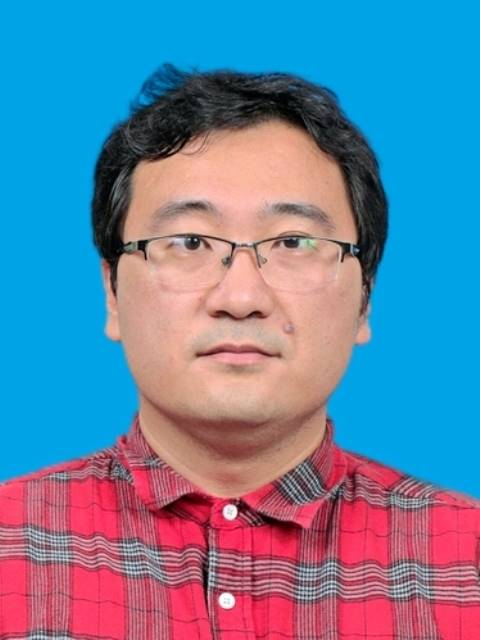
\includegraphics[width=1in,height=1.25in,clip,keepaspectratio]{assets/thales.jpg}}]{Tai Jiang}
  received the master’s degree in Master of Business Administration from the University of Chinese Academy of Sciences, Beijing, in 2022, where he is currently pursuing the Ph.D. degree with the Institute of System Engineering, Macau University of Science and Technology, Macao, China.
  
  he is with the Department of Engineering Science, Faculty of Innovation Engineering, Macau University of Science and Technology, Macao, 999078, China. His research interests include parallel intelligence, blockchain, DAOs, NFTs, Meta, and Decentralized Science.
\end{IEEEbiography}

\vspace{-33pt}

\begin{IEEEbiography}[{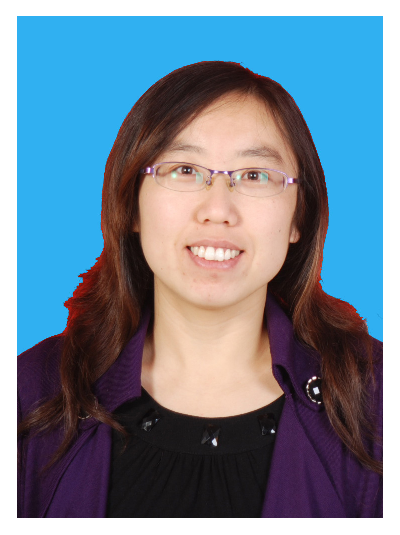
\includegraphics[width=1in,height=1.25in,clip,keepaspectratio]{assets/Rui.eps}}]{Rui Qin}
  (Member, IEEE) received the Ph.D. degree in computer application technology from the University of Chinese Academy of Sciences, Beijing, China, in 2016.

  She is currently an Associate Professor with the State Key Laboratory for Management and Control of Complex Systems, Institute of Automation, Chinese Academy of Sciences, Beijing. Her research interests include blockchain, DAO, and parallel management.
\end{IEEEbiography}

\vspace{-33pt}

\begin{IEEEbiography}[{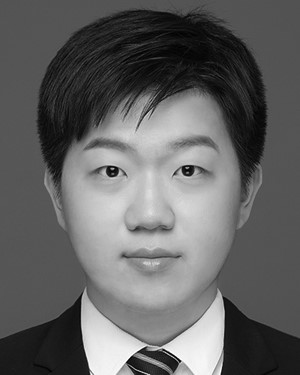
\includegraphics[width=1in,height=1.25in,clip,keepaspectratio]{assets/yhliu.jpg}}]{Yuhang Liu}
  received the B.S. degree from the Department of Precision Instruments, Tsinghua University, Beijing, China, in 2021. He is currently working toward the Ph.D. degree with the Institute of Automation, Chinese Academy of Sciences, Beijing. His research interests include parallel radars, 3D object detection, and point cloud data generation.
\end{IEEEbiography}

\vspace{-33pt}

\begin{IEEEbiography}[{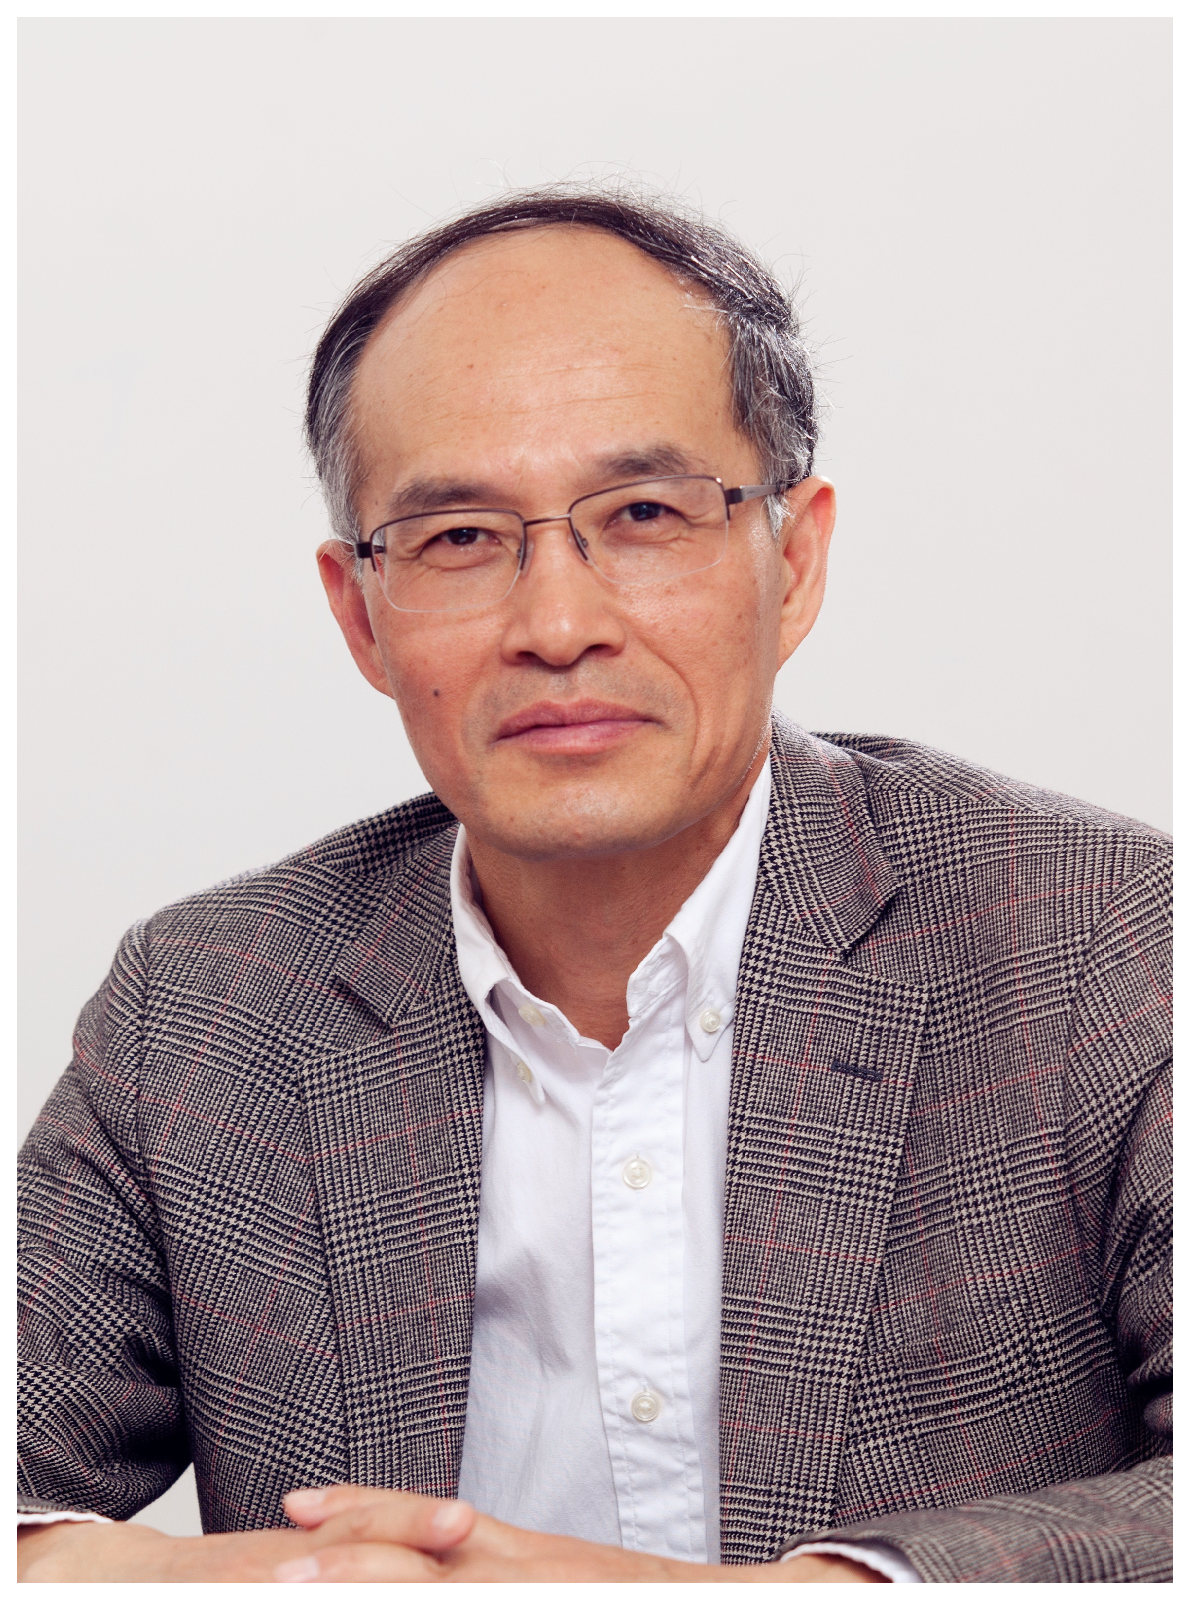
\includegraphics[width=1in,height=1.25in,clip,keepaspectratio]{assets/FW.eps}}]{Fei-Yue Wang} (S’87–M’89–SM’94–F’03)
received his Ph.D. degree in computer and systems engineering from the Rensselaer Polytechnic Institute, Troy, NY, USA, in 1990. He joined The University of Arizona in 1990 and became a Professor and the Director of the Robotics and Automation Laboratory and the Program in Advanced Research for Complex Systems. In 1999, he founded the Intelligent Control and Systems Engineering Center at the Institute of Automation, Chinese Academy of Sciences (CAS), Beijing, China, under the support of the Outstanding Chinese Talents Program from the State Planning Council, and in 2002, was appointed as the Director of the Key Laboratory of Complex Systems and Intelligence Science, CAS, and Vice President of Institute of Automation, CAS in 2006. He found CAS Center for Social Computing and Parallel Management in 2008, and became the State Specially Appointed Expert and the Founding Director of the State Key Laboratory for Management and Control of Complex Systems in 2011. He is a distinguished professor at the Macau University of Science and Technology.

His current research focuses on methods and applications for parallel intelligence, social computing, and knowledge automation. He is a Fellow of International Council on Systems Engineering (INCOSE), International Federation of Automatic Control (IFAC), American Society of Mechanical Engineers (ASME), and American Association for the Advancement of Science (AAAS). In 2007, he received the National Prize in Natural Sciences of China, numerous best papers awards from IEEE Transactions, and became an Outstanding Scientist of Association for Computing Machinery(ACM) for his work in intelligent control and social computing. He received the IEEE Intelligent Transportation Systems (ITS) Outstanding Application and Research Awards in 2009, 2011, and 2015, respectively, the IEEE Systems, Man, and Cybernetics Society (SMC) Norbert Wiener Award in 2014, and became the IFAC Pavel J. Nowacki Distinguished Lecturer in 2021.

Since 1997, he has been serving as the General or Program Chair of over 30 IEEE, Institute for Operations Research and the Management Sciences (INFORMS), IFAC, ACM, and ASME conferences. He was the President of the IEEE ITS Society from 2005 to 2007, the IEEE Council of Radio Frequency Identification (RFID) from 2019 to 2021, the Chinese Association for Science and Technology, USA, in 2005, the American Zhu Kezhen Education Foundation from 2007 to 2008, the Vice President of the ACM China Council from 2010 to 2011, the Vice President and the Secretary General of the Chinese Association of Automation (CAA) from 2008 to 2018, the Vice President of IEEE SMC from 2019 to 2021. He was the Founding Editor-in-Chief (EiC) of the International Journal of Intelligent Control and Systems from 1995 to 2000, IEEE ITS Magazine from 2006 to 2007, JOURNAL OF AUTOMATICA SINICA (IEEE/CAA) from 2014-2017, China's Journal of Command and Control from 2015-2021, and China's Journal of Intelligent Science and Technology from 2019 to 2021. He was the EiC of the IEEE Intelligent Systems from 2009 to 2012, IEEE TRANSACTIONS on ITS from 2009 to 2016, IEEE TRANSACTIONS ON COMPUTATIONAL SOCIAL SYSTEMS from 2017 to 2020. Currently, he is the President of CAA's Supervision Council, and the EiC of IEEE Trans. on Intelligent Vehicles.
\end{IEEEbiography}



\vfill

\end{document}


